
\section{Gothenburg --- Gothenburg Congestion Tax}

\subsection{Implementation}

The most recent place to adopt zone pricing has been Gothenburg---Sweden's second largest city. The infrastructure deal that Stockholm obtained from its Congestion Tax attracted the attention of Gothenburg's leadership, who in 2009 negotiated a 3.4 billion EUR package funded partly by a zone pricing scheme \citep{Borjesson2015}. The outcome of that deal, the Gothenburg Congestion Tax, launched in January 2013. In September 2013, a non-binding public consultation showed 57\% of Gothenburg voters opposed the Tax, but the scheme has been kept in order to fulfill the terms of the infrastructure agreement. \citet{Borjesson2015} attribute the unpopularity of the Congestion Tax to revelations that the infrastructure it purchases---especially a massive underground rail tunnel---will be significantly less beneficial and more expensive than  advertised. 

\subsection{Design}

Gothenburg's scheme was based on Stockholm's. Cameras identify drivers crossing in either direction a cordon around the city center (see Figure \ref{fig:Gothenburg-map}). The toll schedule has the same structure as in Stockholm, though shifts occur 30 minutes earlier, and rates differ slightly at certain times. 

As a city, Gothenburg differs critically from Stockholm. Gothenburg is less than half the size of Stockholm and has less transit usage: in 2012 public transit accounted for 26\% of trips among OD pairs involving the congestion tax in Gothenburg, while the statistic for Stockholm is 77\% \citep{Borjesson2015}. Also, since the CBD is not on a penninsula, Gothenburg has 38 gantries to Stockholm's 18, and several must be situated in residential neighborhoods in order to prevent traffic from diverting onto quiet streets. The ``single charge rule'' states that, no matter how many times a vehicle traverses the cordon within 60 minutes, it is charged only once \citep{transportstyrelsen2015}. In this case, the amount of the toll is the highest among the applicable traversals.

\begin{figure}[ht]
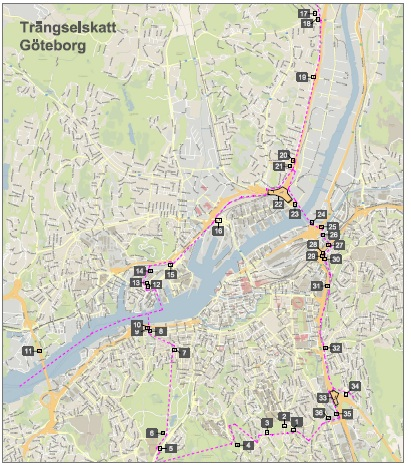
\includegraphics[]{../img/gburg-congestion-tax-map.jpg}

\caption{Gothenburg Congestion Tax zone \citep{transportstyrelsen2015}\label{fig:Gothenburg-map}}
\end{figure}

\subsection{Results}

The effects in Gothenburg were qualitatively similar to but milder than those observed in Stockholm. Traffic over the cordon during the charged hours fell 12\%, rather than the 15\% forecast by models \citep{Borjesson2015}. The discrepancy was largest during the peaks: whereas models had predicted peak travel would fall 18\%, it fell only 13\%---approximately the same reduction observed for off-peak traffic. Travel surveys show that commuters switched to public transport, while discretionary travelers traveled less frequently or switched destinations. Accounting for external factors, the charge is estimated to have raised public transport ridership by about 4.5-6.5\%. As for congestion, Figure \ref{fig:Gothenburg-travel-times} shows travel times in Gothenburg for different classes of road from before and after the charge. Likewise, in Stockholm commuters switched to public transport, public transport ridership rose by about 5\%, discretionary travelers canceled trips, peak and off-peak traffic fell by similar amounts and travel time reductions were strongest on inner arterial roads.

\begin{figure}[ht]
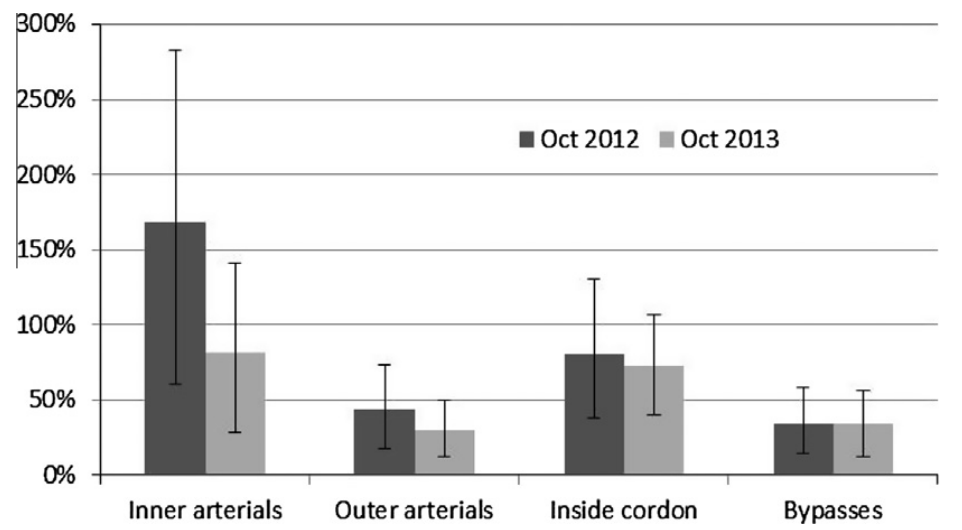
\includegraphics[width=0.55\columnwidth]{../img/gburg-travel-times.png}

\caption{Gothenburg 7-8AM. Increase in travel times on selected categories of road relative to free-flow speeds, before (Oct 2012) and after (Oct 2013) the Congestion Tax. \citep{Borjesson2015} \label{fig:Gothenburg-travel-times}}

\end{figure}

\subsection{Finances}

In 2013 the Gothenburg Congestion Tax raised 846 million kr, of which 76 million kr came from tolls and 83.8 million kr from penalties \citep{TransportstyrelsenGburg2013}. This was short of the 930 million kr (\$103 million) forecast, largely because 45\% of traffic turned out to be exempt rather than the 30\% forecast \citep{Borjesson2015}.

\section{Discussion}\label{sec:discussion}

This chapter has reviewed the history of zone pricing from its conception as an idea in the 1950's and 1960's to its proliferation in the new millenium as a result of number-plate recognition technology. Surveying the zone pricing experience, two themes emerge that are worth highlighting.

First, note that all the systems surveyed produced similar traffic reductions, between 10 and 20 percent of all entries. This is surprising given that the amount of money charged varies considerably. In Stockholm, the maximum charge is only about \$3. In London it was about \$18 before the recent devaluation of the pound. Moreoever, the models in Stockholm and Gothenburg were mistaken in that they predicted different traffic reductions in the peak and off-peak, due to the time-varying toll. Instead what was observed is that a similar share of traffic stopped driving at both times of day. As a rule-of-thumb, it might be worthwhile to assume that, in any pre-charging population of drivers, about 10-15\% of drivers are simply unwilling to pay anything to drive, almost regardless of the size of the toll.

Second, while most of the theory of congestion pricing focuses on prices, in practice exemptions are critical. Some of these exemptions---such as those for the handicapped or medical vehicles---are easy to justify by appeals to welfare or social justice. But many exemptions---such as those for taxis or even, in the case of Milan, refrigerated delivery trucks---lack much of a rationale outside politics.
